\documentclass[12pt,fleqn]{article}
\setlength{\parindent}{0pt}
\usepackage{graphicx}
\usepackage{listings}
\usepackage[latin5]{inputenc}
\setlength{\parskip}{8pt}
\setlength{\parsep}{0pt}
\setlength{\headsep}{0pt}
\setlength{\topskip}{0pt}
\setlength{\topmargin}{0pt}
\setlength{\topsep}{0pt}
\setlength{\partopsep}{0pt}
\setlength{\mathindent}{0cm}

\begin{document}
Ders 8

Onceki dersi hatirlarsak iki tarafinda da $k$ olan, girdisi $cos \omega t$
olan bir ODE uzerinde calistik. 

\[ y' + ky = k cos \omega t \]

Cozmek icin problemi kompleks dunyaya getirdik

\[ \tilde{y} + k\tilde{y} = ke^{i\omega t} \]

Sag tarafin kompleks bir sayinin reel bolumu oldugunu farzettik
boylece. Bunu yaptik cunku ustel sayilarin entegralini almak kolay. Cozum

\begin{equation}\label{8eq1}
\tilde{y} = \frac{1}{1+i(w/k)} e^{i\omega t} 
\end{equation}

olmustu, yani cozum sunun reel bolumu olacakti:

\begin{equation}\label{8eq2}
\frac{1}{\sqrt{1+(w/k)^2}} cos(\omega t - \phi) 
\end{equation}

Bu metotu kutupsal metot olarak nitelemistik. 

Kartezyen yontemini kullansaydik (\ref{8eq1}) formulunun hem ust hem alt
tarafini kartezyene, $a+ib$ formuna cevirecektik. Ilk once alti reel yapmak
icin alti ve ustu bolenin tamamlayicisi (conjugate) ile carpalim

\[ \frac{1-i(w/k)}{1+(w/k)^2} (cos \omega t + isin \omega t)\]

Simdi bunun reel kismini alalim. Carpimi yaparken bir yandan da hayali sayi
kismi atiyoruz, iki islemi ayni anda yapiyoruz yani

\[ \frac{1}{1+(w/k)^2} (cos \omega t + \frac{w}{k} sin \omega t )\]

Boylece sonuca eristik. Simdi sonucu kontrol edelim, hem kutupsal hem
kartezyen yonden gelince ayni sonuc erismemiz lazim. Bu sonuc (\ref{8eq2})
ile ayni mi?

Ayni. Kontrol etmek icin bir trigonometrik esitlik (identity) kullanacagiz,
bu tur gecisleri yapabilmek dersimiz icin cok onemli. Gecis genel formuyla
soyle:

\[ a cos \theta + b sin \theta = C cos(\theta - \phi)\]

$C$ ve $\phi$ reel sayilardir. Onlarin hesabinin bir formulu var, onu
hatirlamak yerine su resmi hatirlamak daha kolay olacaktir

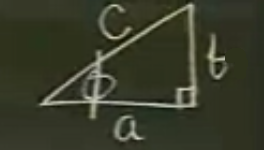
\includegraphics[height=2cm]{8_1.png}

Bizim ornegimiz icin

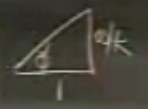
\includegraphics[height=2cm]{8_2.png}

Gecisi yapalim

\[ \frac{1}{1+(w/k)^2} \sqrt{1+(w/k)^2} cos (\omega t - \phi) \]

\[ \phi = tan^{-1}(w/k) \]

Formulun sol kisminda biraz temizleme yapmamiz mumkun

\[ \frac{1}{1+(w/k)^2} \sqrt{1+(w/k)^2} \]

\[ = \frac{1}{ \sqrt{ \bigg(1+(w/k)^2} \bigg)^2} \sqrt{1+(w/k)^2} \]

Karekokler artik birlesebilir, icerideki terimler ayni oldugu icin sagdaki
terim yokolur, kare yerine 1 gelir

\[ = \frac{1}{\sqrt{1+(w/k)^2}} \]

o zaman nihai formul

\[ \frac{1}{\sqrt{1+(w/k)^2}} cos (\omega t - \phi) \]

ve bu formul (\ref{8eq2}) ile aynidir.

Trigonometrik gecisin ispatlari:

Ispat 1

Vektorel olarak dusunursek

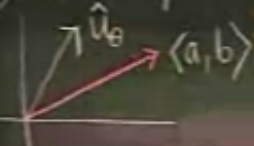
\includegraphics[height=2cm]{8_3.png}

$<a,b>$ bir vektor olarak dusunuluyor, $\hat{u}_\theta$ ise birim vektor,
icerigi $<cos \theta, sin \theta>$. Nasil birim peki? Cunku $cos^2\theta +
sin^2\theta = 1$ 
degerini verir.

Boylece $a cos \theta + b sin \theta$ formulunu iki vektorun nokta carpimi
(dot product) olarak gorebiliriz, yani $<a,b> \cdot <cos \theta, sin
\theta>$. 
Bu formu yazinca noktasal carpimlarin diger tanimina ziplayabiliriz.

\[ <a,b> \cdot <cos \theta, sin \theta> \]

\[ = |<a,b>| \cdot 1 \cdot cos(\theta - \phi) \]

\[ = |<a,b>| \cdot cos(\theta - \phi) \]

Bu formul noktasal carpimin tanimindan ileri geliyor, $x \cdot y =
|x|\cdot|y| \ cos \beta$, $\beta$ iki vektor arasindaki aci. $\theta -
\phi$ cunku iki vektor arasindaki aci boyle.

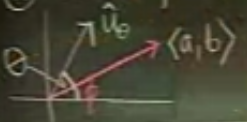
\includegraphics[height=2cm]{8_4.png}

1 degeri ile carpildi, cunku birim vektorun buyuklugu (magnitude) 1
degerindedir. $|<a,b>| = \sqrt{a^2+b^2}$ demektir, yani resimde $C$ olarak
gosterilen seydir. Boylece ispati tamamlamis olduk. 

Ispat 2

Bu ispat kompleks sayilari kullanacak. $a cos \theta + b sin \theta$
formulunu, reel kismi esit olacak sekilde, alttaki sekilde temsil
edecegiz. Stratejimiz o noktadan kutupsal forma atlamak, sonra onun reel
kismini ilk formulumuz $a cos \theta + b sin \theta$ ile karsilastirmak
olacak. 

\begin{equation}\label{eq3}
(a - bi) (cos \theta + i sin \theta) 
\end{equation}

Soldaki eksi isaretinin sebebi bariz, cunku sagdaki eksi ile carpilinca
$i^2 = -1$ ile beraber artiya donusmesi icin. Simdi parca parca kutupsal
forma gecelim. $(a-bi)$ nasil kutupsal forma gecer? $(a+bi)$ arasindaki aci
$\phi$ ise, $(a-bi)$ arasindaki aci $-\phi$ olur. Ikinci kisim zaten
$e^{i\theta}$'dir. Hep beraber

\[ = \sqrt{a^2+b^2}e^{-i\phi} e^{i\theta}\]

\[ = \sqrt{a^2+b^2} e^{i(\theta - \phi) }  \]

Formul (\ref{eq3})'un reel kismini alirsak, $a cos \theta + b sin \theta$
elde ederiz. Ustteki son formulun reel kismi nedir? 

\[ = \sqrt{a^2+b^2}e^{i(\theta - \phi)}\]

\[ = \sqrt{a^2+b^2}cos(\theta - \phi) + isin(\theta - \phi) \]

Reel kismi

\[ \sqrt{a^2+b^2}cos(\theta - \phi)\]

Yani gecisi tekrar ispatlamis olduk. 

Hoca kompleks sayi sisteminin kullanilmasina cok vurgu yapiyor. Dersi
ogretirken bir anlamda matematik alaninin yasadiklarini tekrar yasatiyor
ogrencilere, matematikcilerin kompleks sayi sistemine alismasi icin 300
kusur sene gecti, eger ogrencileri uc hafta bu konuda harcarsa bu pek agir
bir yuk sayilmamali.

Simdi lineer formullere geri donecegiz. Daha onceki derslerde genelden
ozele gecmistik, simdi ters yonde gidelim. 

Temel Lineer ODE

\[1. \  y' + ky = kq_e(t) \] 

En ozel formullerden biri olan bu formul �s� / konsantrasyon ya da aktarma
/ difuzyon (conduction / diffusion) formulu idi.

Fakat fizik basta olmak uzere pek cok alanda $k$ sabitinin sag tarafta
olmayabilecegi durumlar da olacaktir. Bunlardan da bahsetmek gerekir.

\[ 2. \ y' + ky = q(t) \]

Nihayet en genel durumlardan birinde $k$'nin sabit olmadigi durumdur.

\[ 3. \ y' + p(t)y = q(t) \]

Bu formu tanimsiz entegral kullanarak cozmeyi biliyoruz, dersin basinda
bunu islemistik zaten.

Bu ODE'leri cozerken cok onemli bir irdeleme, karar ani $k$'nin eksi mi
arti mi olduguna baglidir. Simdiye kadar hep $k>0$ oldugunu farzettik. 

Karisim Problemi

Hacmi $V$ olan bir icine $r$ hizinda sivi gelen bir kap dusunelim. $x(t)$:
kaptaki $t$ anindaki tuz miktari, $C_e$ gelen sivinin tuz konsantrasyonu. 

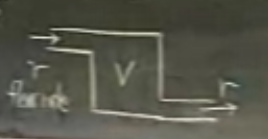
\includegraphics[height=2cm]{8_5.png}

\[ \frac{dx}{dt} = \textrm{ gelen tuz h�z� - giden tuz h�z� } \]

Hiz niye boyle temsil edildi? Hizi olcmek icin iki zaman araliginda yapilan
olcumlerin farkini zaman araligina boleriz. Ustteki formulde, sol tarafta
bu zaman araligi en kucuk (infinitesimal) kesit olacak sekilde
hesaplaniyor, bu yuzden sol tarafta diferansiyel form var. 

\[ = r C_e - r \frac{x}{V} \]

Sivinin gelis hizi $r$'nin hem gidis hem gelis icin kullanildigina dikkat
edelim, kap tamamen dolu, o yuzden gelen sivi oraninda sivi mutlaka disari
cikmali. 

Standart lineer form

\[ \frac{dx}{dt} + \frac{rx}{V} = rC_e(t) \]

\[ C(t) = \frac{x}{V} \]

Iki tarafin diferansiyelini alirsak

\[ \frac{dC}{dt} = \frac{1}{V}\frac{dx}{dt}\]

\[ V\frac{dC}{dt} = \frac{dx}{dt}\]

Buna gore ana diferansiyel denklemdeki formul soyle degisir

\[ V \frac{dC}{dt} + rC = rC_e\]

Standart forma koyalim. Bunu yaparken $r$'nin degil, $r/V$'nin kritik oge
oldugunu goruyoruz.

\[ \frac{dC}{dt} + \frac{r}{V} = \frac{r}{V} C_e \]

Bu formulde tuz miktari yerine konsantrasyon bagimli degiskendir, ve
formulun bu halinin ustteki listede 1. form kategorisine girdigini
goruyoruz. Tabii konsantrasyon derken (biraz kelimeler karismis olabilir),
aktarma / difuzyon modelinden bahsediyoruz aslinda. 

Ve aktarma problemindeki akiskanlik sabiti $r/V$, sadece $r$ degil. $r$
hacim / dakika, $V$ hacim, o zaman $r/V$ 1/dakika, yani $\textrm{dakika}^{-1}$ olur. 

Ornek

Diyelim ki $C_e$ sinussel, $cos \omega t$. Eger $k$ cok buyuk ise, $C(t)$,
$C_e(t)$'yi ne kadar yakinda takip eder? Aktarma probleminden biliyoruz ki
eger akiskanlik sabiti buyukse ic �s� d�s �s�y� yakindan takip
eder. Difuzyonda ayni durum. 

Bizim problemimize bu nasil tercume edilir? Eger $r$ cok buyukse (hizli
akis) o zaman icerideki konsantrasyon disa oldukca yakin olur. Ya da $V$
cok kucuktur, o zaman da kap hizla bosalacaktir, yine ayni durum
olur. Sezgizel olarak anlamli bir sey yani.

Bu demektir ki gecikme (lag) $\phi$ kucuktur, buyukluk (amplitude) ise 1'e
yakindir. 

Bu dersin geri kalaninda 1. formulun, hatta bazen 2. formulun nerede ise
yaramadigina bakalim. 

2'nin isledigi durumlar:

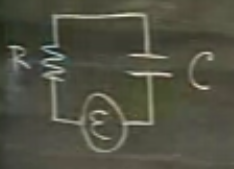
\includegraphics[height=2cm]{8_6.png}

$q$ kapasitorun uzerindeki yuk (charge). 

\[ \frac{dq}{dt} = i \]

Dikkat, ``i'' burada kompleks sayi degil, akim. 

Kirchoff Kanununa gore

\[ R\frac{dq}{dt} + \frac{q}{C} = \varepsilon(t) \]

Standart forma koyarsak

\[ q' + \frac{q}{RC} = \frac{\varepsilon}{R} \]

Bu formulu 1. forma yaklastirmak icin $k=RC$ diye kabul edip, sonra sag
tarafi $k$'lestirmek icin $\varepsilon \cdot C$ almaya ugrasmak gibi
numaralar yapilabilir, fakat bu oldukca dogal olmayan bir yaklasimdir, yani
bu formul 1'de ziyade 2. form ile cozulur. 

Diger bir ornek, zincirleme radyoaktif curumesi (radioactive chain decay). 

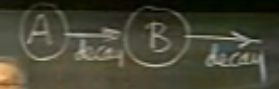
\includegraphics[height=2cm]{8_7.png}

A ve B adinda iki element var (bunlar periyodik tablodaki elementlerden),
ve A curuyor, B oluyor, sonra B curumeye devam ediyor. Basitlik icin tek A
atomu tek B atomuna donusuyor diyelim. Curume nedir? Atomun parcalarini
kaybetmektir, bu sebeple element degisimi olur. Elimdeki ne kadar B
oldugunu merak ediyorum mesela, soyle modelleyebilirim 

\[ \frac{dB}{dt} = k_1 A - k_2 B\]

\[ = k_1A_0 e^{-k_1t} - k_2B \]

Ufak bir yer degisiminden sonra diff denklem 

\[ B' + k_2 B = k_1A_0 e^{-k_1t}\]

Fakat buna bakinca anliyoruz ki $A_0$ sabitinin $k$ sabitinin hicbir
alakasi yok. Bu sebeple ustteki denklem 1. forma uygun degil, dogal
durmuyor. Bu ornekte de 2. form dogru olandir. 

Simdi ufak bir kotu haber: Eger $k < 0$ ise, simdiye kadar gordugumuz
terminolojideki gecici (transient), istikrarli konum (steady-state), girdi
(input), cevap (response) sozlerinin hicbiri gecerli olmaz. Denklemi
``cozme'' yontemi aynidir, mesela

\[ \frac{dy}{dt} - ay = q(t)\]

yani $a > 0$ ve $k < -a$

O zaman cozum olan su formul

\[ e^{-kt} \int q(t) e^{kt} dt + ce^k\]

su hale gelecektir

\[ e^{at} \int q(t) e^{-at} dt + ce^{at}\]

Ne oldu? $a>0$ oldugu icin $ce^{at}$ sonsuzluga gider, bilahere tum cozum
sonsuzluga gider, $c < 0$ ise eksi sonsuzluga gider. O zaman bu kisim
gecici (transient) degil, cunku sifira gitmiyor, ve ne olacagi baslangic
sartlarina cok bagli. Kiyasla $k>0$ oldugu diger durumda gormustuk ki
baslangic sartlarinin ne oldugu hic farketmiyordu. 

Hangi bilim dallarinda $k > 0$ ya da $k < 0$. 

Biyolojide, ekonomide cogunlukla $k < 0$. 

Fizikte cogunlukla $k > 0$. Hocanin esprisi yasamayan seyler varsa $k > 0$,
yasayan seyler varsa $k < 0$. 

\end{document}
